% Created 2022-08-16 mar 18:05
% Intended LaTeX compiler: pdflatex
\documentclass[12pt]{article}
\usepackage[utf8]{inputenc}
\usepackage[T1]{fontenc}
\usepackage{graphicx}
\usepackage{grffile}
\usepackage{longtable}
\usepackage{wrapfig}
\usepackage{rotating}
\usepackage[normalem]{ulem}
\usepackage{amsmath}
\usepackage{textcomp}
\usepackage{amssymb}
\usepackage{capt-of}
\usepackage{hyperref}
\newcommand{\tagline}{Práctica 1}
\newcommand{\asignatura}{Organización de Computadoras (331)}
\newcommand{\docente}{Arturo Arreola Alvarez}
\usepackage[spanish]{babel}
\usepackage{geometry}
\geometry{ a4paper, left=.75in, right=.75in, top=1in, bottom=1in }
\makeatletter
\renewcommand\familydefault{\sfdefault}
\usepackage{sectsty}
\sectionfont{\normalfont\huge}
\subsectionfont{\normalfont\huge}
\usepackage{fancyvrb}
\setcounter{secnumdepth}{1}
\author{Luis Eduardo Galindo Amaya \\
1274895}
\date{2022-08-14}
\title{Elementos en la Organización de una \\
Computadora de Propósito General}
\hypersetup{
 pdfauthor={Luis Eduardo Galindo Amaya \\
1274895},
 pdftitle={Elementos en la Organización de una \\
Computadora de Propósito General},
 pdfkeywords={},
 pdfsubject={},
 pdfcreator={Emacs 26.3 (Org mode 9.1.9)}, 
 pdflang={Spanish}}
\begin{document}

\begin{titlepage}
  \vspace*{0.75in}
  \begin{flushleft} 
	\sffamily      
    
	\large
    \tagline \\

	\Huge
    \@title \\
    \vspace{0.25in}
    \hline
    \vspace{0.25in}
	% \vspace{0.50in}

    \Large
    \@author
    
    
    \vspace*{\fill}
	
    \large
    \begin{tabular}{ |l|l| }
      \hline
      Asignatura & \asignatura \rule{0pt}{15pt}\\
      Docente & \docente \rule{0pt}{15pt}\\
      Fecha & \@date \rule{0pt}{15pt}\\
      \hline
    \end{tabular} \\
\end{titlepage}

\setlength\parindent{0pt}   % eliminar el intentado
\setlength{\parskip}{0.75em}   % expandir el espacio entre párrafos
\vspace*{0.75in}

\section{Intrucciones}
\label{sec:org99f41ba}
El alumno se familiarizará con la herramienta Marie.js para la ejecución de código en lenguaje ensamblador.

\begin{enumerate}
\item Identificar las caracteristicas de la herramienta marie.js
\begin{itemize}
\item Ingrese a la página donde se encuentra la herramienta.
\item Consulte la documentación y tutoriales de Marie, en especial las secciones Introduction to Marie y Marie Codes.
\end{itemize}

\item Realizar los programas
\begin{itemize}
\item solicite al usuario 2 números y despliegue el resultado de la ecuación \(2x+3y-5\).
\item solicite 2 números y los reste. Desplegar un 1 si el resultado fue negativo o un 0 en caso contrario.
\end{itemize}

\item Realizar un reporte que incluya: 
\begin{itemize}
\item Diagrama de bloques de una máquina de von Neumann y una breve descripción de cada componente.
\item Lista de las instrucciones de Marie y su y su función.
\item Describir el funcionamiento de los registros del Acumulador, Registro de instrucción, Contador del Programa, Registro de Acceso a Memoria (MAR), y Registro de Buffer de Memoria (MBR).
\end{itemize}
\end{enumerate}

\pagebreak

\section{Máquina De Von Neumann}
\label{sec:org50141f6}
\begin{description}
\item[{Memoria}] Son un conjunto de celdas usadas para cualquier proceso, se utiliza para almacenar los programas que va a ejecutar el procesador e información que el programa necesite almacenar.

\item[{Unidad Aritmético Lógica}] es un circuito digital electrónico que realiza las operaciones aritméticas y lógicas bit a bit en números binarios enteros.

\item[{Unidad de Control}] es un componente que dirige las operaciones del procesador. Le dice a la memoria, ALU y los dispositivos de entrada y salida cómo responder a las instrucciones de un programa.

\item[{Entrada/Salida}] Es la comunicación entre la computadora y un humano u otro sistema de procesamiento de información. Inputs son las señales o datos recibidos por el sistema y outputs son las señales o datos enviados por éste.

\item[{Registros}] son unidades de almacenamiento pequeñas que son típicamente dirigidas por mecanismos distintos de la memoria principal y a los que se puede acceder más rápido.
\end{description}

\begin{center}
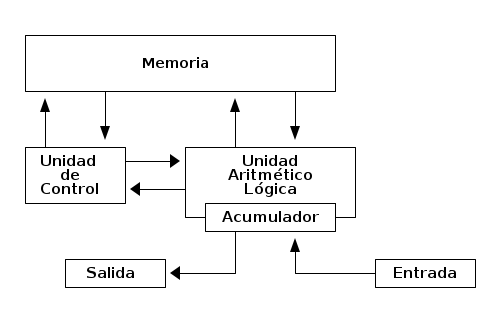
\includegraphics[width=9cm]{./img/maquina-von-neumann2.png}
\end{center}

\section{Registros}
\label{sec:orgbce3bdd}
\begin{description}
\item[{Program counter (PC)}] Registro contador del programa, contiene la dirección de la instrucción siguiente que hay que leer de la memoria.

\item[{Instruction register (IR)}] El registro de instrucción, contiene la instrucción que hay que ejecutar.

\item[{Memory address register (MAR)}] Registro de direcciones de memoria, donde ponemos la dirección de memoria a la que queremos acceder.

\item[{Memory buffer register (MBR)}] Registro de datos de memoria; registro donde la memoria deposita el dato leído o el dato que queremos escribir.

\item[{Acumulador (AC)}] el acumulador es un registro en el que son almacenados temporalmente los resultados aritméticos y lógicos intermedios que serán tratados por el circuito operacional de la unidad aritmético-lógica.
\end{description}

\pagebreak

\section{Instrucciones de Marie.js}
\label{sec:org7b485e4}
\begin{center}
\begin{tabular}{|c|c|l|l|}
\hline
Dec & Hex & Instrucción & Resumen\\
\hline
0 & 0 & JnS X & Jumps and Store: Stores value of PC at\\
 &  &  & address X then increments PC to X+1\\
\hline
1 & 1 & Load X & Loads Contents of Address X into AC\\
\hline
2 & 2 & Store X & Stores Contents of AC into Address X\\
\hline
3 & 3 & Add X & Adds value in AC at address X into AC\\
\hline
4 & 4 & Subt X & Subtracts value in AC at address X into AC\\
\hline
5 & 5 & Input & Request user to input a value\\
\hline
6 & 6 & Output & Prints value from AC\\
\hline
7 & 7 & Halt & End the program\\
\hline
8 & 8 & Skipcond (C) & Skips the next instruction based on C:\\
 &  &  & if(C)=\\
 &  &  & + 000: Skips if AC < 0\\
 &  &  & + 400: Skips if AC = 0\\
 &  &  & + 800: Skips if AC > 0\\
\hline
9 & 9 & Jump X & Jumps to Address X\\
\hline
10 & A & Clear & AC ← 0\\
\hline
11 & B & AddI X & Add Indirect: Use the value at X as the\\
 &  &  & actual address of the data operand to\\
 &  &  & add to AC\\
\hline
12 & C & JumpI X & Uses the value at X as the address to\\
 &  &  & jump to\\
\hline
13 & D & LoadI & Loads value from indirect address into AC\\
 &  &  & e.g. LoadI addresspointer\\
 &  &  & Gets address value from addresspointer, loads\\
 &  &  & value at the address into AC\\
\hline
14 & E & StoreI & Stores value in AC at the indirect address.\\
 &  &  & e.g. StoreI addresspointer Gets value from\\
 &  &  & addresspointer, stores the AC value\\
 &  &  & into the address\\
\hline
\end{tabular}
\end{center}
\pagebreak

\section{Programas}
\label{sec:org7478fb6}
\begin{Verbatim}[numbers=left, frame=single, label=Programa-1.mas, baselinestretch=1.2, framesep=5mm]
/ Solicite al usuario 2 números y despliegue el resultado de la
/ ecuación 2x+3y-5.

INPUT                            / Captura el valor de X
Store X                          
INPUT                            / Captura un valor de Y
Store Y                          

Clear                            / limpiar Acumulador, hacer AC ← 0

Add X                            / 2x
Add X 
Add Y                            / 3y
Add Y
Add Y
Subt R                           / -5

Output
Halt

X, DEC 0
Y, DEC 0
R, DEC 5
\end{Verbatim}
\pagebreak

\begin{Verbatim}[numbers=left, frame=single, label=Programa-2.mas, baselinestretch=1.2, framesep=5mm]
/ Escriba un código que solicite 2 números y los reste.  Desplegar 
/ un 1 si el resultado fue negativo o un 0 en caso contrario.  

INPUT                            / Captura el valor de X
Store X                          
INPUT                            / Captura un valor de Y
Store Y                          

load X                           / Carga el valor de X en el acumulador
Subt Y                           / Resta el valor de Y a X 

/ Para ese punto, el valor en AC es 'X-Y'

Skipcond 000                     / si AC es mayor o igual a 0 
clear                            / el valor en AC se vuelve 0

Skipcond 400                     / si es diferente a 0
Load verdadero                   / el valor en AC se vuelve 1

Output
Halt

X, DEC 0
Y, DEC 0
verdadero, dec 1
\end{Verbatim}

\pagebreak

\section{Capturas De Pantallas}
\label{sec:org3d49dc0}
\begin{figure}[htbp]
\centering
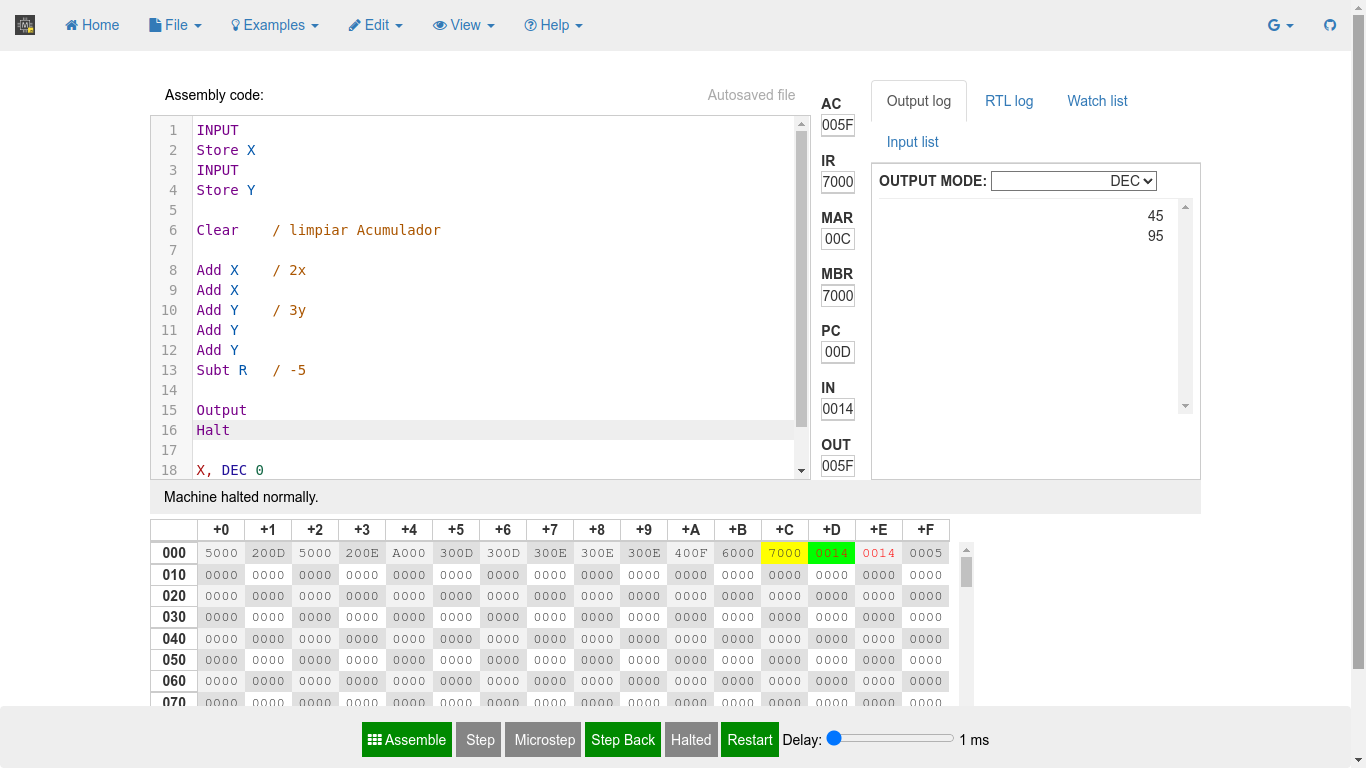
\includegraphics[width=12cm]{img/ddddd.png}
\caption{Ejecución del programa 1}
\end{figure}

\begin{figure}[htbp]
\centering
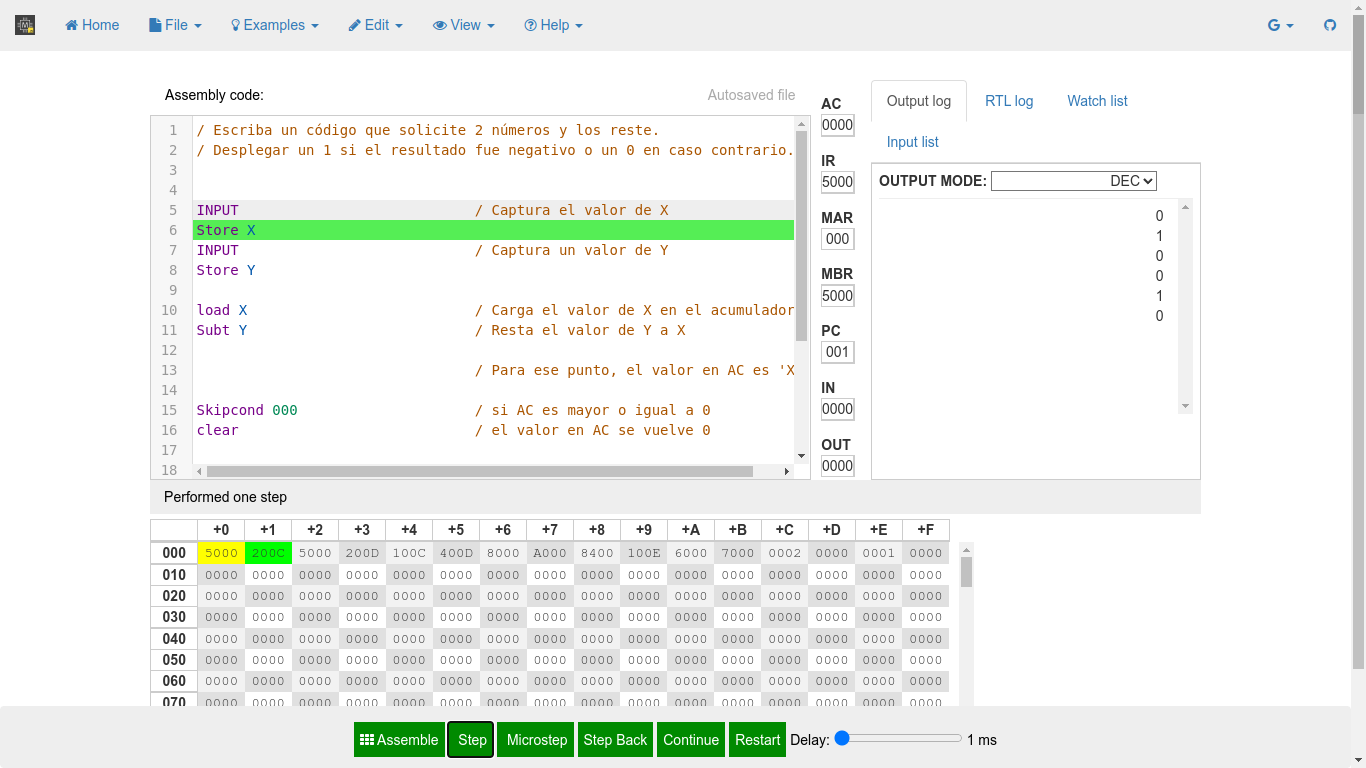
\includegraphics[width=12cm]{img/eeee.png}
\caption{Ejecución del programa 2}
\end{figure}
\pagebreak


\section{Conclusiones y Comentarios}
\label{sec:orgad9517e}
Al programa en ensamblador es necesario estar mas al pendiente de los estados de la memoria al mismo tiempo que las ejecuciones que realizamos, en otras palabras el estado previo de la memoria no puede ser ignorado o extraído para ser procesado.

\begin{description}
\item[{Complicaciones}] En el segundo programa fue necesario que revisara en que orden se tienen que evaluar los operadores  lógicos, ya que si evaluaba primero el '=' no se podía resolver.
\end{description}
\end{document}
